\documentclass{article}
\bibliographystyle{ieeetr}
\usepackage{graphicx} 
\usepackage{svg}

\title{Echocardiography Guidance and Training with Mixed Reality}
\author{Edvart G. Bjerke}
\date{March 2025}

\begin{document}
\maketitle

\section{Introduction}
The aim of this thesis is to implement an echocardiography guidance and training system in augmented reality. The system is targeted at trainees, students and other unskilled practitioners. 
The goal is to provide a tool that is helpful both in learning about how to perform echocardiographic examinations and in actual examinations.

A pre-trained deep neural network- based model will be used to generate guidance signals for the user, and these signals will be integrated into the augmented reality system.  
Additionally, virtual reference model placed in the virtual environment allows the user to explore cardiac structures and familiarize themselves with
standard views. 

The reference models are based on cardiac MRI data. 
Since the project is focused on echocardiography, it's essential that the reference model also includes ultrasound data.
This data should be spatially complete such that the user can view scan planes from arbitrary poses in a continuous manner.
To maintain coherence, all representations (raw MRI, solid model and ultrasound) are obtained from the same patient. 
This ensures that context is not lost when switching between representations.

We wish to investigate whether AR technology coupled with a guidance model can enhance the learning experience of novice echocardiography users.
This thesis hypothesizes that such technologies can reduce friction in the learning experience through increased interactivity and reduction of the context-switching
apparent in traditional learning methods. We propose that providing immediate feedback and displaying information directly in the users field of view 
promotes more focused learning where the need to shift attention, both physically and mentally, is reduced. We also aim to investigate if these techniques 
improve the user's ability to understand and internalize the geometry of cardiac structures.


\section{Research Question and Evaluation Plan}
The following is a preliminary overview of the research question and evaluation plan.

To assess the effectiveness of augmented reality (AR) in echocardiography training, this thesis will investigate 
the following question:

\textbf{How can AR-based guidance improve the learning experience of novice echocardiography users?}
In particular, experiments will focus on whether AR-based guidance leads to faster skill acquisition, 
higher success rates in obtaining diagnostically acceptable views, and improved learner confidence and engagement.

To answer this question, a user study will be conducted comparing two training methods: one based on current standard practice, 
and another using the proposed AR guidance system. Participants will be novice users with limited or no prior echocardiography 
experience, such as medical students or early-stage residents. Participants will be randomly assigned to one of the two groups.

Both groups will be instructed to obtain a set of apical views using a physical ultrasound probe in a simulation setting. 
The AR group will have access to live guidance through the headset, including real-time feedback and visualization 
of target probe positioning. The control group will follow conventional instructional material, 
such as handouts, diagrams, and verbal/written instructions.

Several evaluation metrics will be collected:
\begin{itemize}
    \item \textbf{Time to acquisition:} The time taken to successfully acquire each standard view.
    \item \textbf{View quality:} Expert assessment of the diagnostic acceptability of each view, based on predefined scoring criteria.
    \item \textbf{User feedback:} A post-task survey measuring perceived learning effectiveness, system usability, and subjective confidence.
\end{itemize}

The primary outcome of interest is whether participants in the AR-guided group can learn to obtain standard views more quickly and with higher
accuracy than those in the control group. Secondary outcomes include participant-reported engagement and satisfaction with the training method.

This evaluation plan will provide some quantitative evidence on the pedagogical value of 
our echocardiography guidance system.
Insights from the user study may also inform further system improvements and broader applications in imaging training.

\section{Echocardiography}
Echocardiography examinations provide information about the patient's heart used to diagnose various 
cardiovascular disorders. Today, echocardiography is used extensively, as the procedure is low-cost and non-invasive \cite{Omerovic2023}.
In Transthoracic Echocardiography (TTE), the ultrasound probe is positioned externally- on the chest of the patient.
This is the most common technique for obtaining echocardiograms, and is less invasive than Transesophageal Echocardiography (TEE), where 
a probe is inserted into the esophagus \cite{Omerovic2023}. In this thesis, we are only concerned with TTE.

In echocardiography, ultrasound waves are transmitted by a probe. The waves propagate through the medium of the patient and echoes are recorded
by the probe. These echoes are processed by a set of signal processing algorithms to produce the ultrasound image. A technique known as "beamforming" is an essential part of the ultrasound processing chain. 
There are several imaging \textit{modalities} used in cardiac ultrasound. The most common types are M-mode, 2D and 3D imaging.
An example of 2D and 3D echocardiography is shown in figure \ref{fig:echoExample}

\begin{figure}[tbh!]
    \centering
    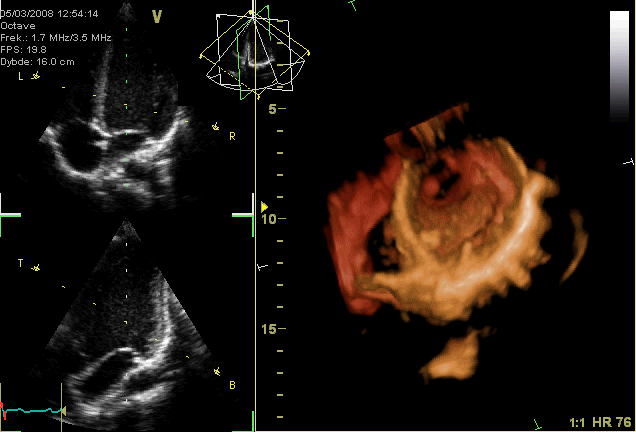
\includegraphics[width=0.65\textwidth]{images/Apikal4D.png}
    \caption{An example of 2D and 3D echocardiography images \cite{lenes2008apikal4d}.}
    \label{fig:echoExample}
\end{figure}

In M-mode imaging, only a single ultrasound scan line is processed and displayed. This modality
may be useful when evaluating the motion or timing of a specific structure with respect to the cardiac cycle \cite{SAUL2015686}.
Two-dimensional ultrasound allows the generation of cross-sectional images of the anatomy.

Three-dimensional ultrasound technology produces volumetric data of the anatomy by using two-dimensional transducer arrays.
These volumes can be produced in real-time and displayed using volume rendering techniques like ray-marching or isosurface generation. One key advantage with 3D echo
is that volumes can be estimated directly from measurements reducing errors intrinsic in volume estimation from cross-sectional slices \cite{Shah2013}.
In this thesis, we are mostly concerned with two-dimensional imaging as this is the most available method.

Beamforming technqiques exploit wave interference to combine ultrasound signals from separate transducers. The result of beamforming is a
greyscale image visualizing anatomical structures. More specifically, the intensity of a pixel in the image correlates with the strength of the reflected echo, influenced by differences
in acoustic impedance.

Due to the intricacies of acoustic wave propagation and limitations in beamforming, ultrasound images are generally more difficult to interpret than those obtained by Computed Tomography or Magnetic Resonance.
These images typically contain significant noise and frequently exhibit visual artefacts such as \textit{abberations} and \textit{reverberations}. Echocardiography is specifically limited due to 
rib blockages, and the probes are designed such that the acoustic field of view may pass in between the ribs of the patient.

\subsection{Standard Viewing Planes}
The standard viewing planes are specific standardized cross-sections used to assess cardiac health.
The standard views are as follows \cite{otto2018echocardiography}:
\begin{itemize}
    \item Parasternal long axis
    \item Parasternal short axis
    \item Apical four-chamber
    \item Apical two-chamber
    \item Subcostal chamber
\end{itemize}

These views are obtained by placing the probe at specific positions and orientations, which requires
training and experience. This paradigm is useful as it provides well-defined goals
for the user to reach and forms a basis for objective assessment of the quality of the examination.

For the scope of this thesis, we choose to only consider views from the apical window.
This is done for simplicity, as all views can then be obtained by rotation of the probe at a single location 
on the thorax.

Views in the apical window are obtained by placing the probe at the \textit{apex} of the left ventricle \cite{otto2018echocardiography}.
With the probe in the correct location for the apical window, all apical views can be obtained by rotating the probe in place
%, as shown in figure \ref{fig:apicalViews}.
% \begin{figure}[h]
%     \centering
%     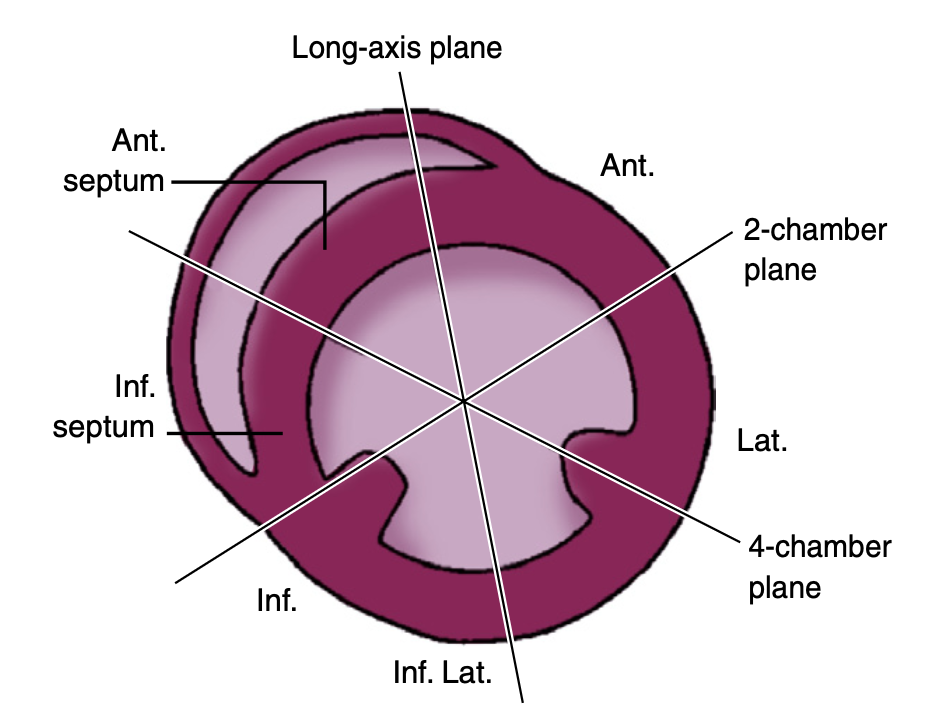
\includegraphics[width=0.5\textwidth]{images/apicalViews.png}
%     \caption{}
%     \label{fig:apicalViews}
% \end{figure}

% \subsubsection{Apical Four-Chamber View}
% The apical four-chamber (A4C) view is obtained by placing the probe at the LV apex.

% typically just lateral to the point of maximal impulse, 
% with the indicator pointing toward the patient's left side or shoulder. 
% The ultrasound beam is directed superiorly, along the long axis of the heart.

% This view simultaneously displays all four cardiac chambers and both atrioventricular valves. 
% It is central to assessing global and relative chamber sizes, systolic function, and valvular motion. 
% In clinical practice, the A4C view is also a primary window for Doppler-based flow measurements, 
% including evaluation of diastolic function and regurgitant flow.

% \subsubsection{Apical Two-Chamber View}

\section{System Architecture and Implementation}
The echocardiography guidance system is implemented as a mixed reality application, integrating several key components:
\begin{itemize}
    \item An ultrasound machine
    \item The Quest 3
    \item A game engine with a custom rendering implementation and AR integration
    \item Virtual anatomical reference models from real patients, with time-varying models acquired by various imaging technologies
    \item A probe position/orientation tracking system
    \item A neural network-based guidance model
    \item A computer with a modern Graphical Processing Unit for rendering and model inference
    \item A hardware/software interaction layer to handle I/O
\end{itemize}

The game engine Unity \cite{unity2025} is chosen for its flexibility in rendering implementation and its AR integration system.
Unity allows for custom shader injection \cite{unityShaders2025} which allows us to add non-standard rendering methods such as 
volumetric ray casting. Also, scripts written in C\# can be used to incorporate custom game/system logic.

The neural network guidance model, implemented in PyTorch \cite{paszke2019pytorch} will receive probe data and the current echo image and predicts adjustments toward a target standard view. 
This prediction is visualized in the AR interface as an arrow or overlay aligned with the user's field of view.
To handle the complexity of hardware, drivers, data transfer and general interoperability in such a complex system, 
ROS (Robot Operating System) \cite{quigley2009ros} will be used.

Extracting data from the ultrasound machine itself will be done using a capture card device.
The images are then distributed within the system with ROS, to be used as input to the guidance model
and for display in the Unity-powered AR system.

The reference models will mainly be represented as surface meshes and scalar fields. These will
be visualized in unity the built-in mesh renderer as well as custom surface and volume renderers.
A custom animation system implementation will also be used to handle smooth rendering of 4D reference models.

To track the position and orientation of the ultrasound probe, AR tags will be used.
AR tags are square fiducial markers in black and white with known patterns and dimensions \cite{nrc_artag}. These markers
are identified in camera images using computer vision techniques and their relative position and orientation
can be computer based on the pixel positions of marker keypoints.






\section{Computer Graphics}
Computer graphics (CG) is the study of digitally generating images, videos, and other types of graphical content.
The type of visual content generated can broadly be categorized into photorealistic and non-photorealistic CG.
The applications of CG techniques are broad- including scientific visualizations, video games, special effects and other types of informative or artistic content.

Algorithms in computer graphics typically operate on objects of a three-dimensional (3D) \textit{scene}. The scene is a high-level description of the virtual environment used to synthesize the visual content.
The objects in the scene may represent things like solid bodies, cameras, light sources or arbitrary volumetric data.

\subsection{Rendering}
Rendering algorithms generate digital images, given a set of objects from the scene. These algorithms
are often physically-based, where \textit{photorealistic} techniques simulate real light phenomena to produce visually realistic results. 


\textit{Non-photorealistic} rendering techniques are used when photorealism is n    ot desired- whether for aesthetic purposes or when the objects represent something
invisible to the human eye. 

\subsection{The Graphics Pipeline}
The graphics pipeline is a high-level description of the sequence of processes used to 
generate an image from the scene description. The graphics pipeline is not rigidly defined,
and different architectures are used to render different tyepes of data or to achieve results of a particular aesthetic.

In real-time computer graphics, the graphics pipeline can generally be viewed as three parts- the application, geometry processing and rasterization \cite{RealTimeRendering}.

\begin{figure}[tbh]
    \centering
    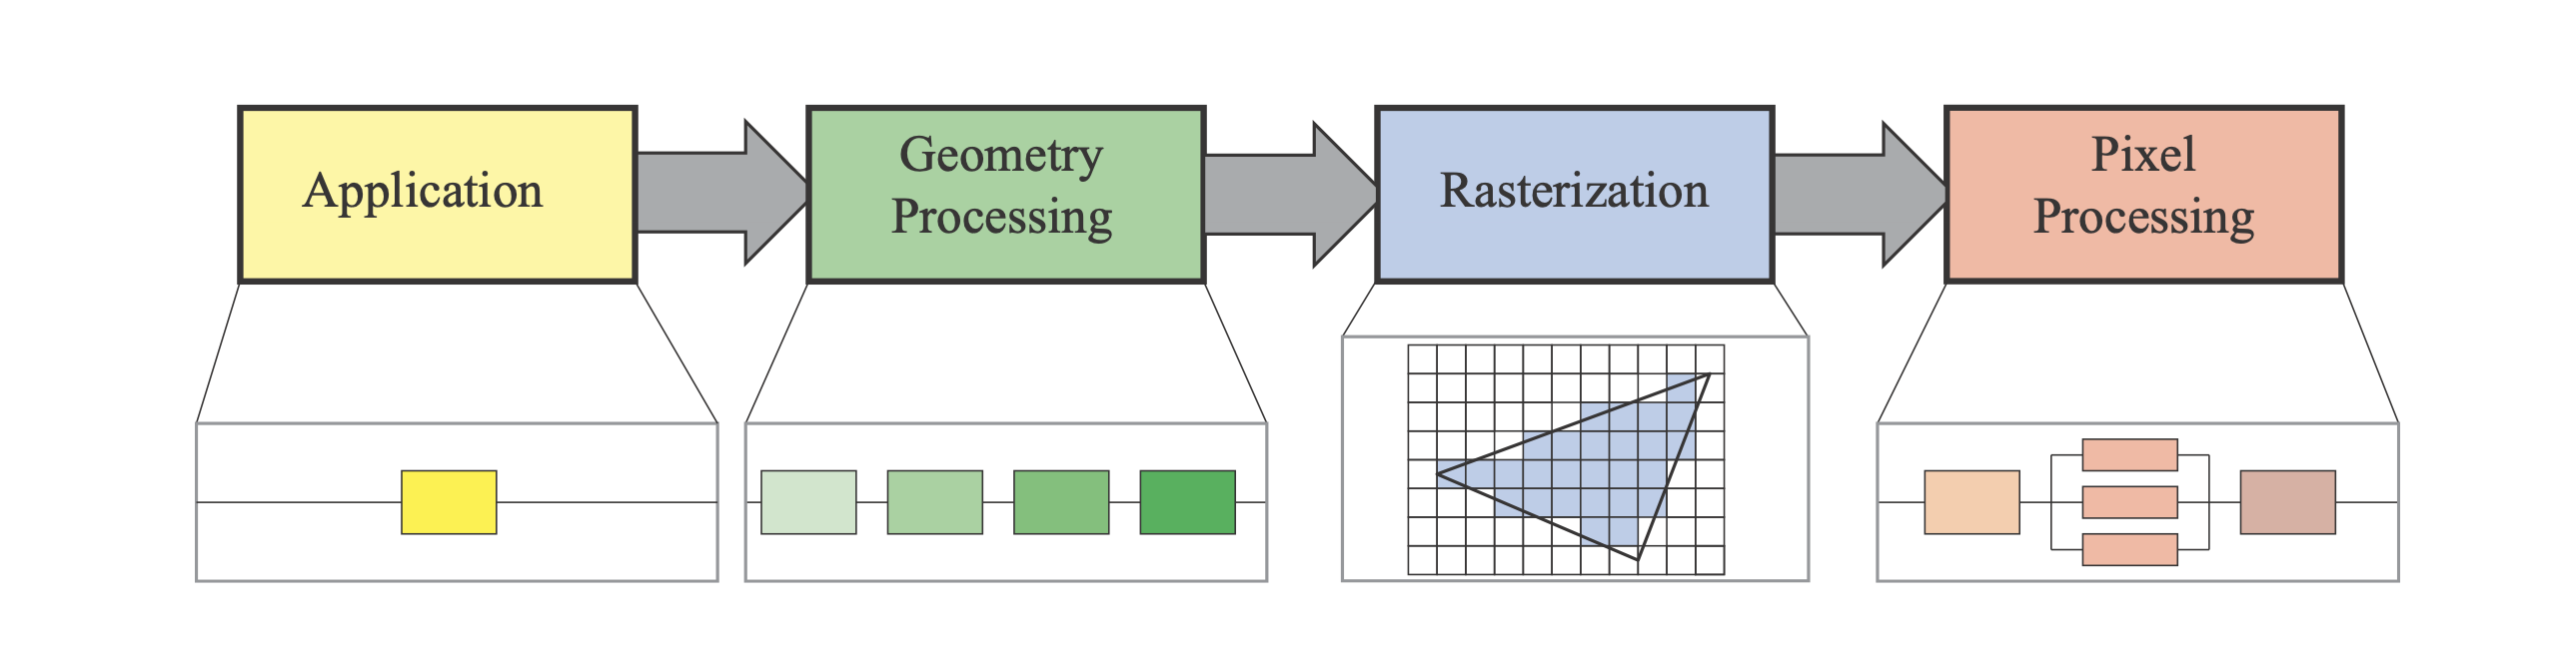
\includegraphics[width=1.0\textwidth]{images/graphics_pipeline.png}
    \caption{The graphics pipeline \cite{RealTimeRendering}}
    \label{fig:pipelineRealTimeRendering}
\end{figure}

The application part of the pipeline generally runs on the CPU, and is concerned with defining the structure of the scene, setting up rendering commands and other pre-processing procedures.
The application defines a set of geometry \textit{primitives} which are sent further down the pipeline. These primitives
are geometrical shapes like triangles and lines, defined by coordinates and indices defining the surface of the models to be processed and rendered by the GPU.
The data strutures representing these primitives are typically defined in a local coordinate system referred to as \textit{object space}, and may include additional information such as surface normals and texture coordinates. The data required
in this stage depends on the algorithms employed in the \textit{pixel processing} stage of the pipeline.

The geometry processing stage is executed on the GPU, where geometrical operations like morphing and subdividing (tesselation) may be performed.
An essential part of the geometry processing stage is the \textit{vertex shader}, which is a programmable procedure which processes each 3D vertex (position) of the given mesh.

In a typical rendering pipeline, the vertex shader transforms the vertex coordinates from \textit{object space} to \textit{screen space} through perspective projection, such that
objects are correctly rendered to the screen according to the \textit{pinhole camera model}.

\begin{figure}[tbh]
    \centering
    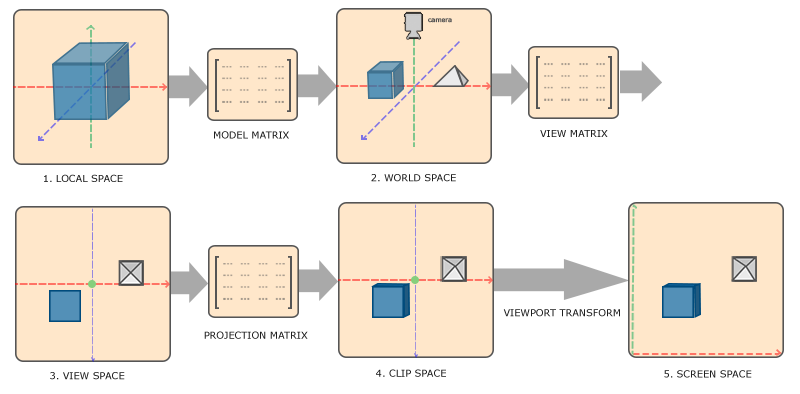
\includegraphics[width=1.0\textwidth]{images/coordinate_systems.png}
    \caption{Representation of geometry processing in a standard vertex shader using perspective projection\cite{learnopengl_figure}.}
    \label{fig:graphicsTransformations}
\end{figure}

The rasterization part of the pipeline uses the screen space coordinates computed by the vertex shader to
determine the set of pixels covered by the projection of the primitive. 

Finally, the colors of the rasterized pixels are determined in the pixel processing stage.
The GPU program defining the algorithm used for shading pixels is referred to as the \textit{fragment shader}.
The fragment shader is executed in parallell, for each rasterized pixel. With modern GPUs and graphics frameworks, fragment shaders are highly programmable, and different shaders may be used to render different objects.

\newpage

\subsection{Volume Rendering}
The traditional raster-based rendering technique is not well-suited for rendering phenomena that are volumetric in nature.
Special rendering techniques have been developed to render physically occuring phenomena like smoke, clouds or fog. These techniques
may also be used to visualize three-dimensional scientific data, like that captured by fluid simulation or medical imaging.

\begin{figure}[tbh]
    \centering
    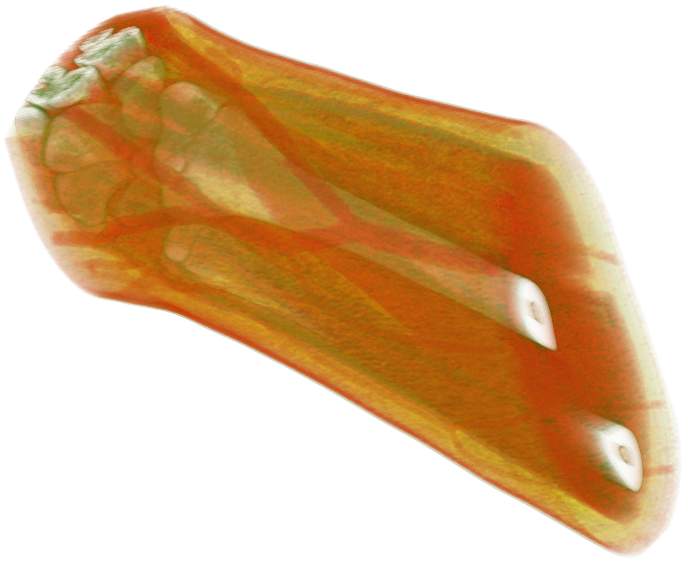
\includegraphics[width=0.5\textwidth]{images/VolumeRendering.png}
    \caption{Volume rendering of a CT scan of a forearm}
    \label{fig:forearmCT}
\end{figure}

\subsubsection{Cut Planes}
A simple way to render volumetric data is reduce the problem to two dimensions, by only rendering a single \textit{slice} of the data
at once. This can be achieved by rendering a plane placed such that it intersects with the bounding volume of the 
data set. 
\begin{figure}[tbh!]
    \centering
    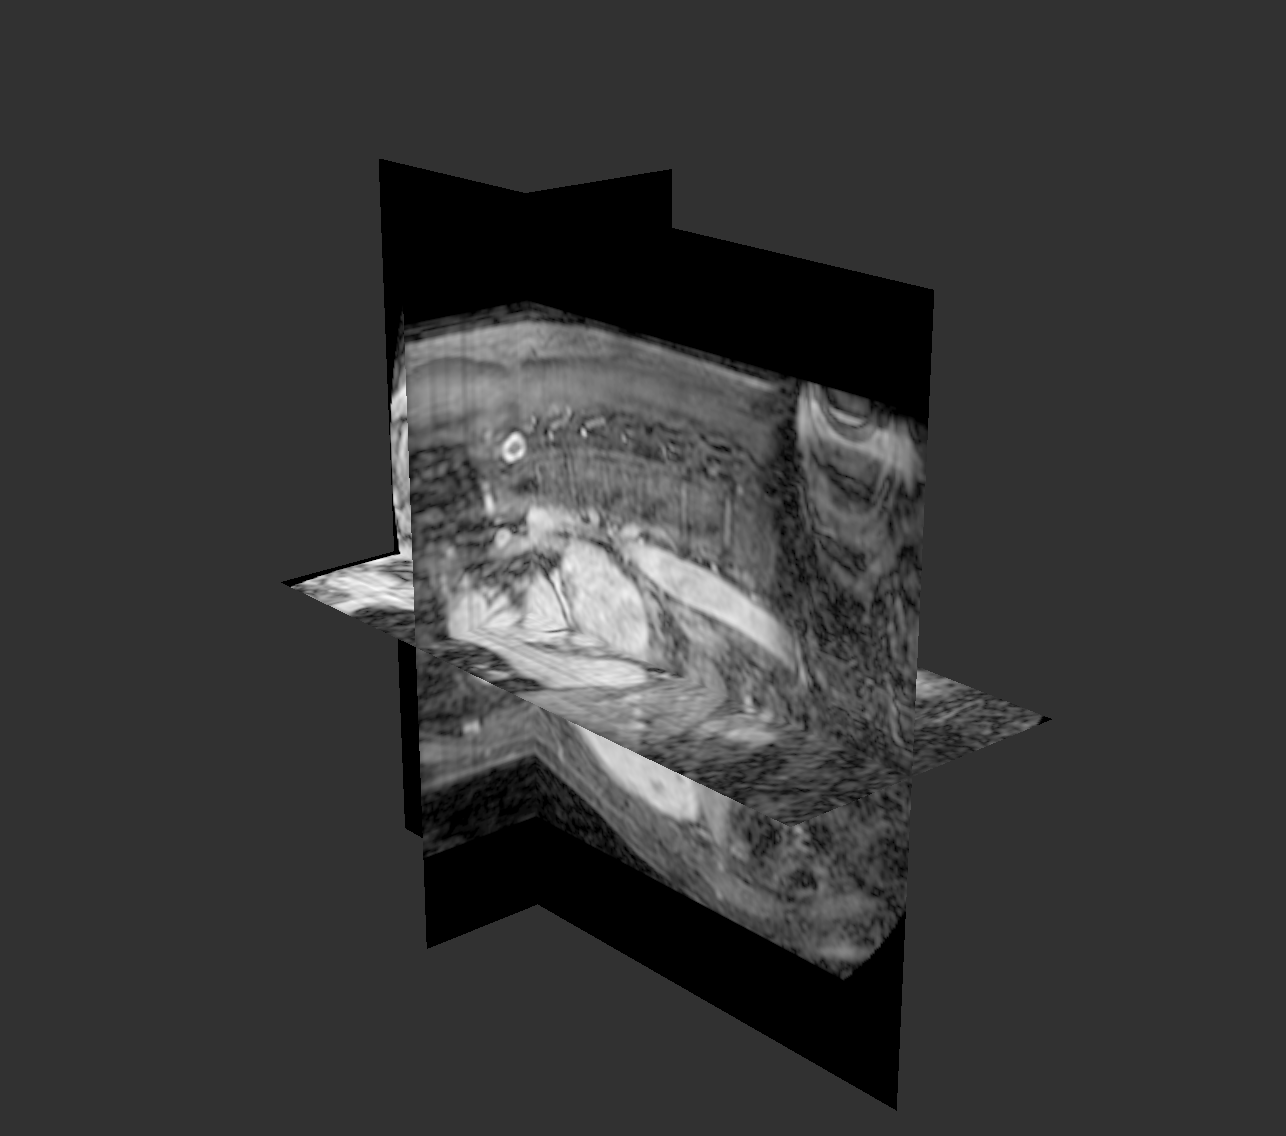
\includegraphics[width=0.53\textwidth]{images/CutPlanes.png}
    \caption{Volume rendering of an MRI dataset using three cut planes.}
    \label{fig:cutPlanes}
\end{figure}
In the fragment shader, the world space position of each fragment is used to sample the volumetric data set. The sampled value can then be used to determine the final color of the pixel via some transfer function.
This method is interpret and implement in the rasterization pipeline, requiring only a simple modification to the fragment shader. 

\subsubsection{Volume Ray Casting}
Volume Ray Casting is a rendering technique used to directly render volumetric scalar fields.
Intuitively, a ray is projected from each pixel into the volume,
and the scalar field is iteratively sampled along each ray to compute the pixel values.
This algorithm approximates the volume rendering rendering integral by computing the Discrete Volume Rendering Integral (DVRI) 

$$ I(D) = \sum_{i=0}^n C_iA_i\prod_{j=i+1}^{n}(1-A_j)$$
Where $I$ is the accumulated intensity for a given pixel with total ray depth $D$.
$C_i$ and $A_i$ represent the intensities and opacities sampled along the ray, respectively. This
can be extended to color images by performing the same algorithm for each channel in the color image (RGB).

If ray-casting is performed front-to-back, the algorithm takes the following form \cite{Kruger2006GPU}
$$ C_{dst} \leftarrow C_{dst} + (1-\alpha_{dst})C_{src} $$
$$ \alpha_{dst} \leftarrow \alpha_{dst} + (1-\alpha_{dst})\alpha_{src}$$
Here, the \textit{destination} color $C_{dst}$ and opacity $A_{dst}$ are computed by 
\textit{compositing} the result from the previous iteration with the \textit{source} values, sampled at the current ray segment. To sample arbitrary positions with the volume, trilinear interpolation is used. A shading model may also be applied during ray traversal,
and this typically requires computing the gradients of the scalar field.

Transfer functions are used to map data values from the 3D scalar field to colors and opacities. The choice of transfer function
depends on the desired visualization and may require expert insight into the nature of the underlying data.
The steps of the volume ray casting algorithm are demonstrated in figure \ref{fig:volumeRayCasting}.


\begin{figure}[tbh]
    \centering
    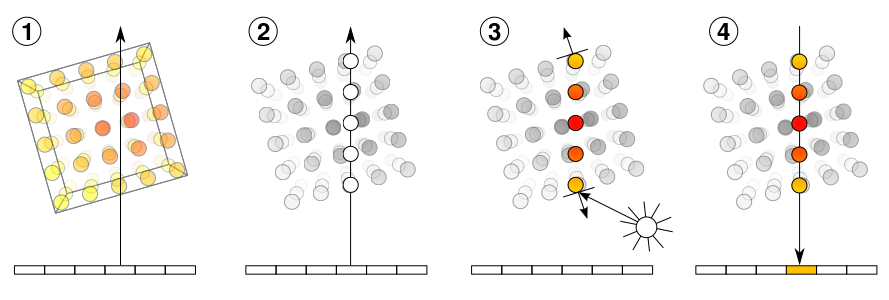
\includegraphics[width=0.9\textwidth]{images/Volume_ray_casting.png}
    \caption{Volume ray casting. The generated ray for a given fragment is shown in (1), passing through the discrete scalar field. In (2), data values are sampled along the ray. Then, a transfer function and shading model are applied at each sample (3) to compute color and opacity values. Finally, the pixel value
    is computed through compositing (4) \cite{Hofmann2011}.}
    \label{fig:volumeRayCasting}
\end{figure}

This algorithm can be implemented on the GPU by conforming to the traditional rasterization pipeline by using \textit{proxy geometries}.
The proxy geometries are placed such that the rasterized pixels cover the projection of the scalar field in view space. Thus,
the ray casting algorithm can be implemented directly in the fragment shader used for these geometries. 

\subsection{Isosurface Rendering}
In isosurface rendering, a triangulated mesh is generated directly from the volume data.
The mesh is formed by generating vertices at volume cells whose data includes a specific value.
This value is refered to as the \textit{isovalue}
The mesh can then be rendered using the traditional rasterization pipeline for rendering surfaces, and 
lighting models can be applied to achieve proper shading. This method is generally cheaper in rendering cost as the
geometry is directly rendered through projection and rasterization rather than by direct volume rendering such as with
ray casting.

A well-known isosurface generation technique for scalar fields is the marching cubes algorithm \cite{lorensen1987marching}.
This algorithm generates coherent 3D surface meshes from 3D scalar fields and is often used for visualization of medical imaging
data such as that obtained by MRI. An example visualization is shown in figure \ref{fig:marchingCubesMRI}

\begin{figure}[tbh]
    \centering
    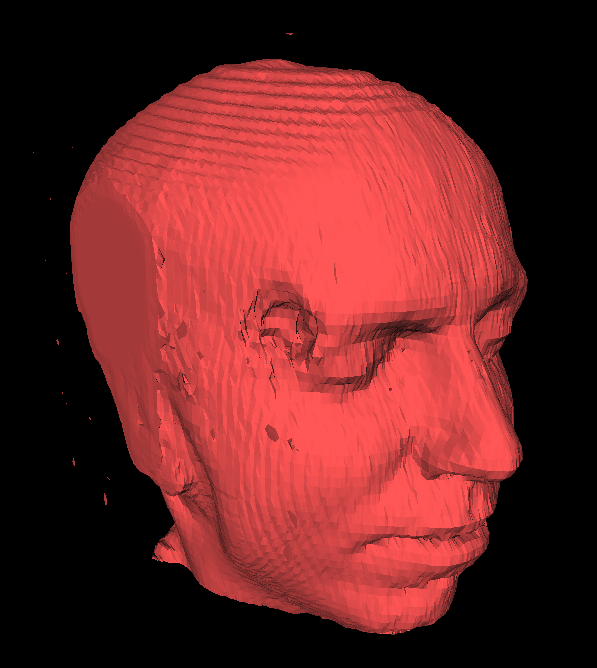
\includegraphics[width=0.5\textwidth]{images/Marchingcubes-head.png}
    \caption{A visualization of a mesh generated by the marching cubes algorithm on MRI data of a human head.}
    \label{fig:marchingCubesMRI}
\end{figure}


\bibliography{references}
\end{document}
